\documentclass[10pt,a4paper]{ULBreport}
\usepackage[utf8]{inputenc}
\sceau{pic/official_logos/sceauULB.png}
\graphicspath{ {./pic/} }
\usepackage{multirow}
\usepackage{listings}
\usepackage{color} 
\usepackage{setspace} 
\usepackage{amsmath}
\usepackage{hyperref}
\usepackage{pdfpages}
\usepackage{biblatex}
\usepackage{floatrow}
\usepackage{subcaption} 
\usepackage{siunitx}
\usepackage[many]{tcolorbox}
\usepackage{multirow}
\usepackage{listings}
\usepackage[dvipsnames]{xcolor}
\usepackage{fancyvrb}

\usepackage{xstring}
\usepackage{etoolbox}

% Colors

\definecolor{darkerGreen}{HTML}{53850d}

% BOXES FOR QUESTIONS

\newtcolorbox{Task}[2][]{
    fontupper=\bf,
    boxrule=1.5pt,
    colframe= black, % frame color
    fonttitle=\itshape,
    attach boxed title to top left={yshift=-0.3\baselineskip-0.4pt,xshift=2mm},
    title= #2,#1,
    enhanced,
    }

\begin{document} 


	\titleULB{
	title={Lab report},
    studies={IRELE},
    course ={Advanced Measurement and Data Driven Modelling},
    author={\textit{Author:} \\ Colot Emmeran},
    date={\textbf{Academic year:} \\ 2024 - 2025},
    teacher={\textit{Professor: } \\ J. Lataire \\ \textit{TA: } \\F. Vandeputte},
    logo={pic/official_logos/logos.jpg},
    manyAuthor
	}

%\listoftables % ToC for tables

%\listoffigures % ToC for figures

\chapter{Lab 1: RLS with forgetting factor}

\section{Main steps}

\begin{enumerate}
    \item Measure the input and output signals from the DUT. The input is arbitrary and the time varying part of the system is due to a manual switch.
    \item Make a first estimate of the parameters with an LLS estimator
    \item Use the RLS estimator with forgetting factor to track the time-varying parameters of the system.
    \item Deduce from the estimated parameters the time instants at which the system changes.
\end{enumerate}

\section{Time-varying RLS estimation}

Starting from the recursive equation of the system, a matrix formulation is derived:

\begin{align}
    y(N) &= b_0(N) u(N) + b_1(N) u(N-1) - a_1(N) y(N-1) - a_2(N) y(N-2) \\
    &= K(N) \theta(N)
\end{align}

with
\begin{align}
    K(N) = \begin{bmatrix} u(N) & u(N-1) & -y(N-1) & -y(N-2) \end{bmatrix}, \hspace{1cm}
    \theta(N) = \begin{bmatrix} b_0(N) \\ b_1(N) \\ a_1(N) \\ a_2(N) \end{bmatrix}
\end{align}

The RLS estimator (with forgetting factor) is a recursive algorithm that computes the parameters $\theta (N)$ and their covariance matrix $K_N$ after each new sample is collected. Because it is recursive, it needs to be initialized and this is done with a linear least squares estimate on a few first samples. \\
The linear least squares estimator, used to find $\theta$ in $y_{\text{lls}} = H \theta$, is in our case constructed as follows:

\begin{align}
    H = \begin{bmatrix}
    u(n_{\text{start}} + 1) & u(n_{\text{start}}) & -y(n_{\text{start}}) & -y(n_{\text{start}} - 1) \\
    u(n_{\text{start}} + 2) & u(n_{\text{start}} + 1) & -y(n_{\text{start}} + 1) & -y(n_{\text{start}}) \\
    \vdots & \vdots & \vdots & \vdots \\
    u(n_{\text{LLS}} - 1) & u(n_{\text{LLS}} - 2) & -y(n_{\text{LLS}} - 2) & -y(n_{\text{LLS}} - 3) \\
    \end{bmatrix}, \hspace{1cm}
    y_{\text{lls}} = \begin{bmatrix}
    y(n_{\text{start}} + 1) \\
    y(n_{\text{start}} + 2) \\
    \vdots \\
    y(n_{\text{LLS}} - 1) \\
    \end{bmatrix}
\end{align}



Where $n_{\text{start}} = \max(n_a, n_b)$ and $n_{\text{LLS}}$ is the number of samples used for the LLS estimate, chosen to be 200 here.

$\theta (n_{\text{LLS}})$ and $P_{n_{\text{LLS}}}$ are found with, respectively, the solution to the LLS problem and the definition of the covariance matrix in the RLS algorithm: 

\begin{align}
    \theta (n_{\text{LLS}}) = (H^T H)^{-1} H^T y_{\text{lls}}, \hspace{1cm}
    P_{n_{\text{LLS}}} = (H^T H)^{-1}
\end{align}

The Matlab code of the LLS initialization is given below:
\begin{lstlisting}[language=Matlab, basicstyle=\ttfamily\footnotesize, keywordstyle=\color{blue}, commentstyle=\color{darkerGreen}, stringstyle=\color{red}]
% initialization with an LLS estimate over a few of the first samples
% y_lls = H * theta
H = zeros(sampleForLLS - max(na, nb), na + nb + 1);
for uCol = 0:nb
    H(:, uCol + 1) = u((max(na, nb) + 1 - uCol:sampleForLLS - uCol));
end
for yCol = 1:na
    H(:, nb + 1 + yCol) = -y((max(na, nb) + 1 - yCol:sampleForLLS - yCol));
end
y_lls = y((max(na, nb) + 1:sampleForLLS));

theta = H\y_lls;
P = inv(H'*H);
\end{lstlisting}

The recursive least squares equations with forgetting factor $g$ are given by:
\begin{align}
    \theta (N) &= \theta (N-1) - \frac{P_{N-1} K^T(N) \left[K(N) \theta (N-1) - y(N)\right]}{g + K(N) P_{N-1} K^T(N)} \\
    P_{N} &= \frac{1}{g} \left( P_{N-1} - \frac{P_{N-1} K^T(N) K(N) P_{N-1}}{g + K(N) P_{N-1} K^T(N)} \right)
\end{align}

The Matlab code implementing these equations is given below:
\begin{lstlisting}[language=Matlab, basicstyle=\ttfamily\footnotesize, keywordstyle=\color{blue}, commentstyle=\color{darkerGreen}, stringstyle=\color{red}]

theta_sav = zeros(na + nb + 1, N - max(na, nb) + 2);
P_diag_sav = zeros(na + nb + 1, N - max(na, nb) + 2);

for itr = sampleForLLS+1:N

    % saving previous values
    theta_sav(:, itr - max(na, nb) + 1) = theta;
    P_diag_sav(:, itr - max(na, nb) + 1) = diag(P);

    K_itr = [u(itr - (0:nb)), -y(itr - (1:na))];

    theta = theta - (P * (K_itr') * (K_itr * theta - y(itr))) / (g + K_itr * P * (K_itr'));
    P = 1/g * (P - (P * (K_itr') * K_itr * P) / (g + K_itr * P * (K_itr')));

end
\end{lstlisting}

\section{Results}

The input of the system is not interesting to show here as it is random white noise. The evolution in time of the estimated parameters is however much more interesting:

\textbf{Plot theta(g) for at least 2 experiments}

\textbf{Conclude which g suits the best}

From the results above, we can take as estimated parameters the values just before the switch and at then end of the experiment. Because the system consists of two LTI systems switched manually, the transfer functions of each of them can be deduced from the estimated parameters:

\begin{align}
    G_{low}(z) &= \frac{b_0 z + b_1}{z^2 + a_1 z + a_2} = \frac{0.5 z + 0.15}{z^2 - 0.4 z + 0.05} \\
    G_{high}(z) &= \frac{b_0 z + b_1}{z^2 + a_1 z + a_2} = \frac{0.29 z + 0.27}{z^2 - 1.25 z + 0.8}
\end{align}

and their frequency responses can be plotted as follows:
\begin{figure}[H]
    \centering
    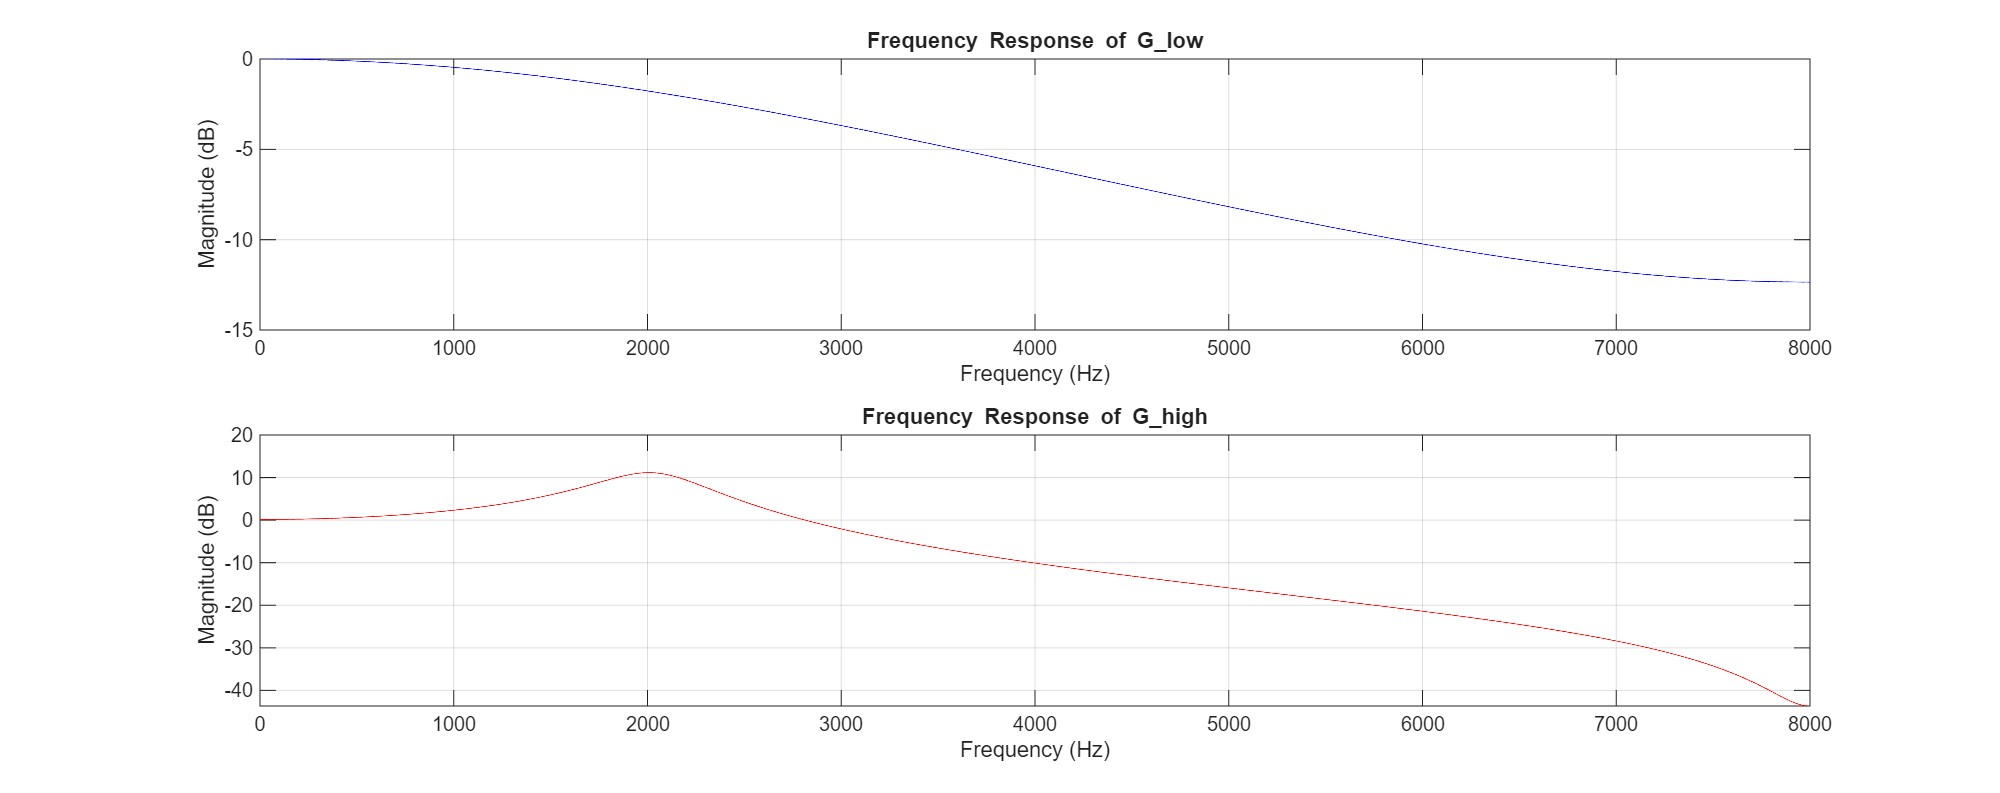
\includegraphics[width=0.8\textwidth]{../matlab scripts/lab1/results/tf_plots.jpg}
    \caption{Frequency responses of the two operating modes of the system}
    \label{fig:lab1_pt3_freq_response}
\end{figure}

\section{Conclusion}

\textbf{See then}






%\printglossary

%\printglossary[type=\acronymtype]

%Bibliography
%\nocite{*}
%\printbibliography[type=article,title=Articles]

\end{document}	